\documentclass[notitlepage, a4paper, 12pt]{report}

\usepackage[utf8]{inputenc}
\usepackage[T1]{fontenc}
\usepackage{ragged2e}
\usepackage{geometry}
\usepackage{graphicx}
\usepackage{setspace}
\usepackage{hyperref}
\graphicspath{{.}}

\newcommand{\ie}{\textit{i}.\textit{e}.}
\renewcommand{\appendixname}{Annexe}

\begin{document}

% ########## TITLE PAGE
\pagestyle{empty}
\centering


\includegraphics[scale=0.75]{Sciences_SU}
\\
\vspace{20mm}
\rule{\textwidth}{0.4pt}
\huge \bf
Waterpixels, des super-pixels respectant les contours des objets dans les images
\rule{\textwidth}{0.4pt}
\\
\vspace{20mm}
\normalsize Auteur : Mathias VELO
\\
\vspace{5mm}
26 mars 2021
\\
\vspace{40mm}
\begin{flushright}
\emph{Encadrante: Isabelle BLOCH}
\end{flushright}

\newpage

% ########## START
\setcounter{page}{1}
\pagestyle{plain}

\begin{flushleft}

\section*{\underline{Présentation}}

Mon sujet porte sur l'implémentation d'une méthode de segmentation d'image nommée \emph{waterpixels}.
\newline
\newline
Ce dont il s'agit quand les termes waterpixels ou superpixels sont employés est une agglomération de pixels connexes, l'image étant ainsi partitionnée en un ensemble de blocs de pixels que l'on appelle waterpixels.
\newline
\newline
On utilise içi en priorité le terme waterpixel à  superpixel, car il fait directement écho à la méthode de segmentation qui est utilisée lors de la dernière étape du traitement subit par une image : l'algorithme de segmentation par ligne de partage des eaux, ou \textbf{watershed segmentation} en anglais.  
\newline
\newline
Ces waterpixels, permettent de partitionner une image de façon assez régulière en suivant les contours des éléments de l'image.
\newline
\newline
La détection de contours est une première étape dans un pipeline de traitement de l'image, pouvant servir entre autres à des applications de vision par ordinateur, dont la reconnaissance faciale et la robotique.
\newline
\newline
Cette première étape de segmentation doit donc être efficiente en temps de calculs, car le résultat de la segmentation n'est pas une fin en soi, mais une première étape vers d'autres traitements successifs.
\newline
\newline
Afin de répondre à cette contrainte, j'ai décidé d'implémenter le code en C++, et de me servir d'OpenCL afin de massivement paralléliser les calculs sur GPU. À défaut de pouvoir me servir de la carte graphique pour certains algorithmes, j'ai fais usage du multithreading sur CPU.

\newpage

Le processus de production des waterpixels se déroule en six étapes:
\begin{enumerate}
\item Chargement d'une image à segmenter
\item Calcul du gradient de l'image
\item Définition d'une grille avec résolution variable, puis sélection de marqueurs dans chaque cellule (en vert sur l'image ci-dessous)
\item Tessellation de Voronoï à partir des marqueurs
\item Combinaison des images aux étapes 2 et 4 (régularisation du gradient)
\item Segmentation par ligne de partage des eaux, sur l'image produite à l'étape 5, à partir des marqueurs de l'étape 3, nous donnant enfin les waterpixels
\end{enumerate}

\begin{figure}[!htb]
\begin{center}
\includegraphics[scale=1.125]{waterpixels_result}
\caption{Étapes du pipeline de production des waterpixels}
\end{center}
\end{figure}

\newpage

\section*{\underline{Recherche documentaire}}

Mes recherches se sont principalement portées sur des aspects techniques, tels que la découverte de l'outil OpenCL[4][5][6] pour les besoins du projet, et la manière dont on passe d'un espace de représentation des couleurs à un autre (espace RGB vers LAB)[2].
\newline
\newline
Je me suis bien évidemment servis du document de référence[1] sur les waterpixels fournis par mon encadrante, et ai consulté une ressource externe sur les "extinction values"[3] en citation de ce document.
\newline
\newline
Pour la conception de l'IHM avec le framework Qt, je me suis simplement servis de la documentation officielle en ligne, à cette adresse : \url{https://doc.qt.io/qt-5/qtgui-module.html}, laquelle listant toutes les classes d'interface utilisateur, et renseignant la manière dont il faut se servir de telle ou telle classe.
\newline
\newline

\section*{\underline{Implémentation}}

Du côté de l'implémentation, j'ai pu coder l'ensemble des fonctions du pipeline de production des waterpixels d'une image.
\newline
Comme dit lors de la présentation du sujet, le code est fait en C++, l'IHM avec Qt, la communication avec le GPU via OpenCL, et la compilation avec CMake.
\newline
\newline
Chacune des étapes de production des waterpixels possède sa propre fonction, aussi ai-je pris le soin de garder en copie chaque image produite par les étapes successives, afin de pouvoir les visualiser dans l'interface via le menu \emph{layer}, lequel permet de montrer ou cacher un calque de rendu associé à une étape de traitement spécifique.
\newline
\newline

\begin{figure}[!htb]
\begin{center}
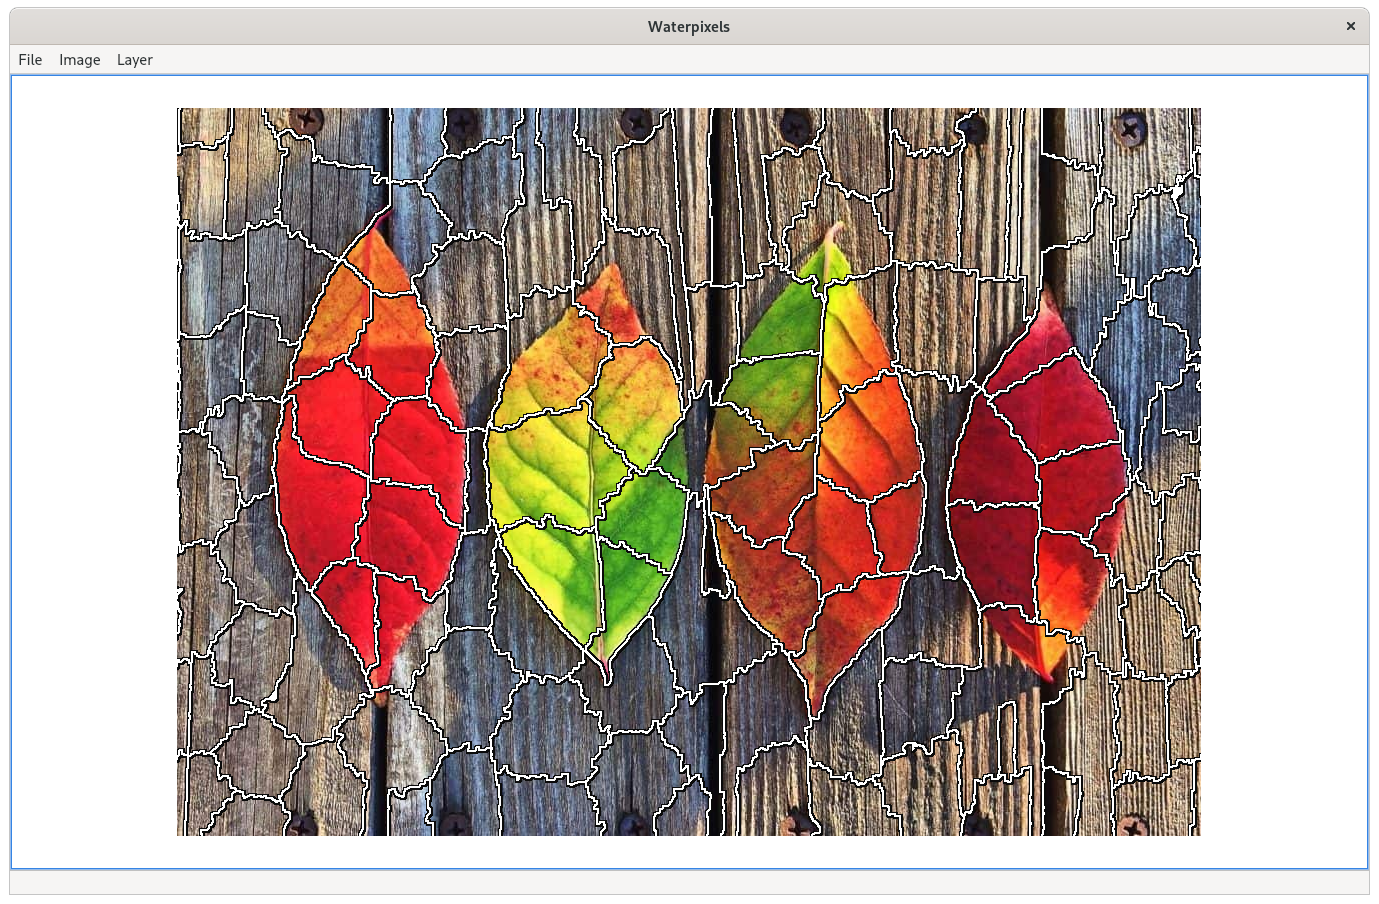
\includegraphics[scale=0.25]{waterpixels_UI}
\caption{Interface utilisateur}
\end{center}
\end{figure}

Une chose que je n'ai pas mentionné concernant le pipeline de production des waterpixels, est l'étape 1.a, qui est donc entre l'étape 1 et l'étape 2, et qui réalise deux opérations morphologiques, une ouverture et une fermeture (forme en croix), ceci afin de faire disparaître les détails de l'image qui sont plus petits que la taille des waterpixels attendus.
\newline
\newline
Pour la suite du projet, il me reste à évaluer les performances de l'outil, aussi bien en terme de temps de calculs, que de la précision des contours obtenus comparativement à une segmentation de référence.
\newline
\newline
Pour l'évaluation des performances sur les temps de calculs, je pense me servir d'un outil de profiling comme gprof sur Linux, que j'ai déjà pu brièvement tester sur le logiciel, et d'un profiler GPU pour les routines OpenCL (peut-être NSight de NVIDIA).
\newline
\newline
Il est aussi demandé d'analyser la régularité des waterpixels, \ie{} si chaque superpixel possède à un écart type près la même densité que les autres waterpixels.

\appendix
\chapter{Bibliographie}

[1] Vaïa Machairas, Matthieu Faessel, David Cárdenas-Peña, Théodore Chabardes, Thomas Walter, et
al.. Waterpixels. IEEE Transactions on Image Processing, Institute of Electrical and Electronics
Engineers, 2015, 24 (11), pp.3707 - 3716. 10.1109/TIP.2015.2451011. hal-01212760

\vspace{3mm}

[2] “Les espaces de couleur RVB et Lab,” Accessed on: Feb. 22, 2021. [Online]. Available: \url{http://www.tsi.enst.fr/pages/enseignement/ressources/beti/RVB_ou_LAB/html/colorspace.html}

\vspace{3mm}

[3]	A. G. Silva et R. d A. Lotufo, « New Extinction Values from Efficient Construction and Analysis of Extended Attribute Component Tree », in 2008 XXI Brazilian Symposium on Computer Graphics and Image Processing, oct. 2008, p. 204‑211, doi: 10.1109/SIBGRAPI.2008.8.

\vspace{3mm}

[4] David Gohara. "Episode 1 - Introduction to OpenCL", YouTube, June. 18, 2013 [Video file]. Available: https://www.youtube.com/watch?v=QA483lIvL-4. [Accessed: Sat. 20, 2021].

\vspace{3mm}

[5] David Gohara. "Episode 2 - OpenCL Fundamentals", YouTube, June. 18, 2013 [Video file]. Available: https://www.youtube.com/watch?v=e-2bTxKuS2U. [Accessed: Sat. 20, 2021].

\vspace{3mm}

[6] David Gohara. "Episode 3 - Building an OpenCL Project", YouTube, June. 18, 2013 [Video file]. Available: https://www.youtube.com/watch?v=yAz9Kj6zRcA. [Accessed: Sat. 20, 2021].

\end{flushleft}


\end{document}
